\documentclass{report}

\usepackage[spanish]{babel}
\usepackage[utf8x]{inputenc}
\usepackage{amsmath}
\usepackage{graphicx}
\usepackage[colorinlistoftodos]{todonotes}
\usepackage{enumitem}
\usepackage{listings}
\usepackage{verbatim}
\usepackage{eurosym}
\usepackage[export]{adjustbox}
\usepackage{amssymb}
\usepackage{bussproofs}
\usepackage{amsmath}
\usepackage{tikz}
\usepackage{xcolor}
\usepackage{listings}
\usepackage{titletoc}
\usepackage{hyperref}

\hypersetup{
  colorlinks=true,
  linkcolor=black,
  urlcolor=blue,
  citecolor=black
}

\newcommand{\coverPage}[6]{%
%----------------------------------------------------------------------------------------
%	COVER START
%----------------------------------------------------------------------------------------
\begin{titlepage}

    \newcommand{\HRule}{\rule{\linewidth}{0.5mm}}
    \newcommand{\department}{#1}
    \newcommand{\course}{#2}
    \newcommand{\titleValue}{#3}
    \newcommand{\subtitleValue}{#4}
    \newcommand{\authorName}{#5}

    \center

    %----------------------------------------------------------------------------------------
    %	HEADER
    %----------------------------------------------------------------------------------------
    
\includegraphics{images/logo_usa.png}
    \vspace{0.5cm}
    \textsc{\Large \department}\\[0.5cm]
    \textsc{\Large \course}\\[0.5cm]
    \vfill

    %----------------------------------------------------------------------------------------
    %	TITLE
    %----------------------------------------------------------------------------------------

    \HRule\\
    \Huge
    \textbf{\titleValue}\\[0.5cm]
    \Large
    \textbf{\subtitleValue}\\
    \HRule\\[0.5cm]

    %----------------------------------------------------------------------------------------
    %	AUTHOR AND DATE
    %----------------------------------------------------------------------------------------

    \vfill
    \Large
    \textit{\authorName}\\
    {\large \today}\\[2cm]

\end{titlepage}
%----------------------------------------------------------------------------------------
%	COVER END
%----------------------------------------------------------------------------------------
}

\begin{document}
    \coverPage{ Matemáticas }{ Introducción al Cálculo }{ Parcial }{ Polinomios }{ Alexander Mendoza }{\today}
    \tableofcontents

    \pagebreak
    \chapter{ Parcial }

    \section*{Polinomios}.
        Sea $P(x) = 2x^3 - 5x^2 - 4x +3$
        \begin{enumerate}
            \item Liste todos los posible ceros raiconales de $P$.\\
                Sabemos que por el teorema de los zeros racionales los posibles ceros de un polinomio son dados por las fracciones que se pueden formar con el coeficiente líder y la constante donde el denominador es un factor del coeficiente líder y el numerador un factor de la constante. Por lo tanto los posibles ceros del polinomio $P$ son:

                $P.R.R = \{ \pm \frac{3}{2}, \pm 3, \pm \frac{1}{2}, \pm 1 \}$
            \item Encuentre la factorización completa de $P$.
            \item Determine los ceros de $P$.\\
                Realizando division sintética con $-1$ logramos conseguir una de las tres raíces.

                \[
                \begin{array}{c|ccccc}
                -1 & 2 & -5 & -4 & 3 & 0 \\
                \hline
                &  & -2 & 7 & -3  \\
                \end{array}
                \]

                Luego el polinomio restante sería $2x^2 - 7x + 3$. Aplicando fórmula cuadrática tenemos que los ceros restantes son.
                \begin{align*}
                    x &= \frac{-(-7) \pm \sqrt{(-7)^2 - 4(2)(3)}}{2(2)} \
                    &= \frac{7 \pm \sqrt{49 - 24}}{4} \
                    &= \frac{7 \pm \sqrt{25}}{4} \
                    &= \frac{7 \pm 5}{4}
                \end{align*}
                Así los ceros del polinomio serían. $-1,\frac{1}{2},3$. Y su forma factorizada sería $(x +1 )(x-3)(x - \frac{1}{2})$\\\\
            \item Bosqueje la gráfica de $P$.\\
                \begin{center}
                    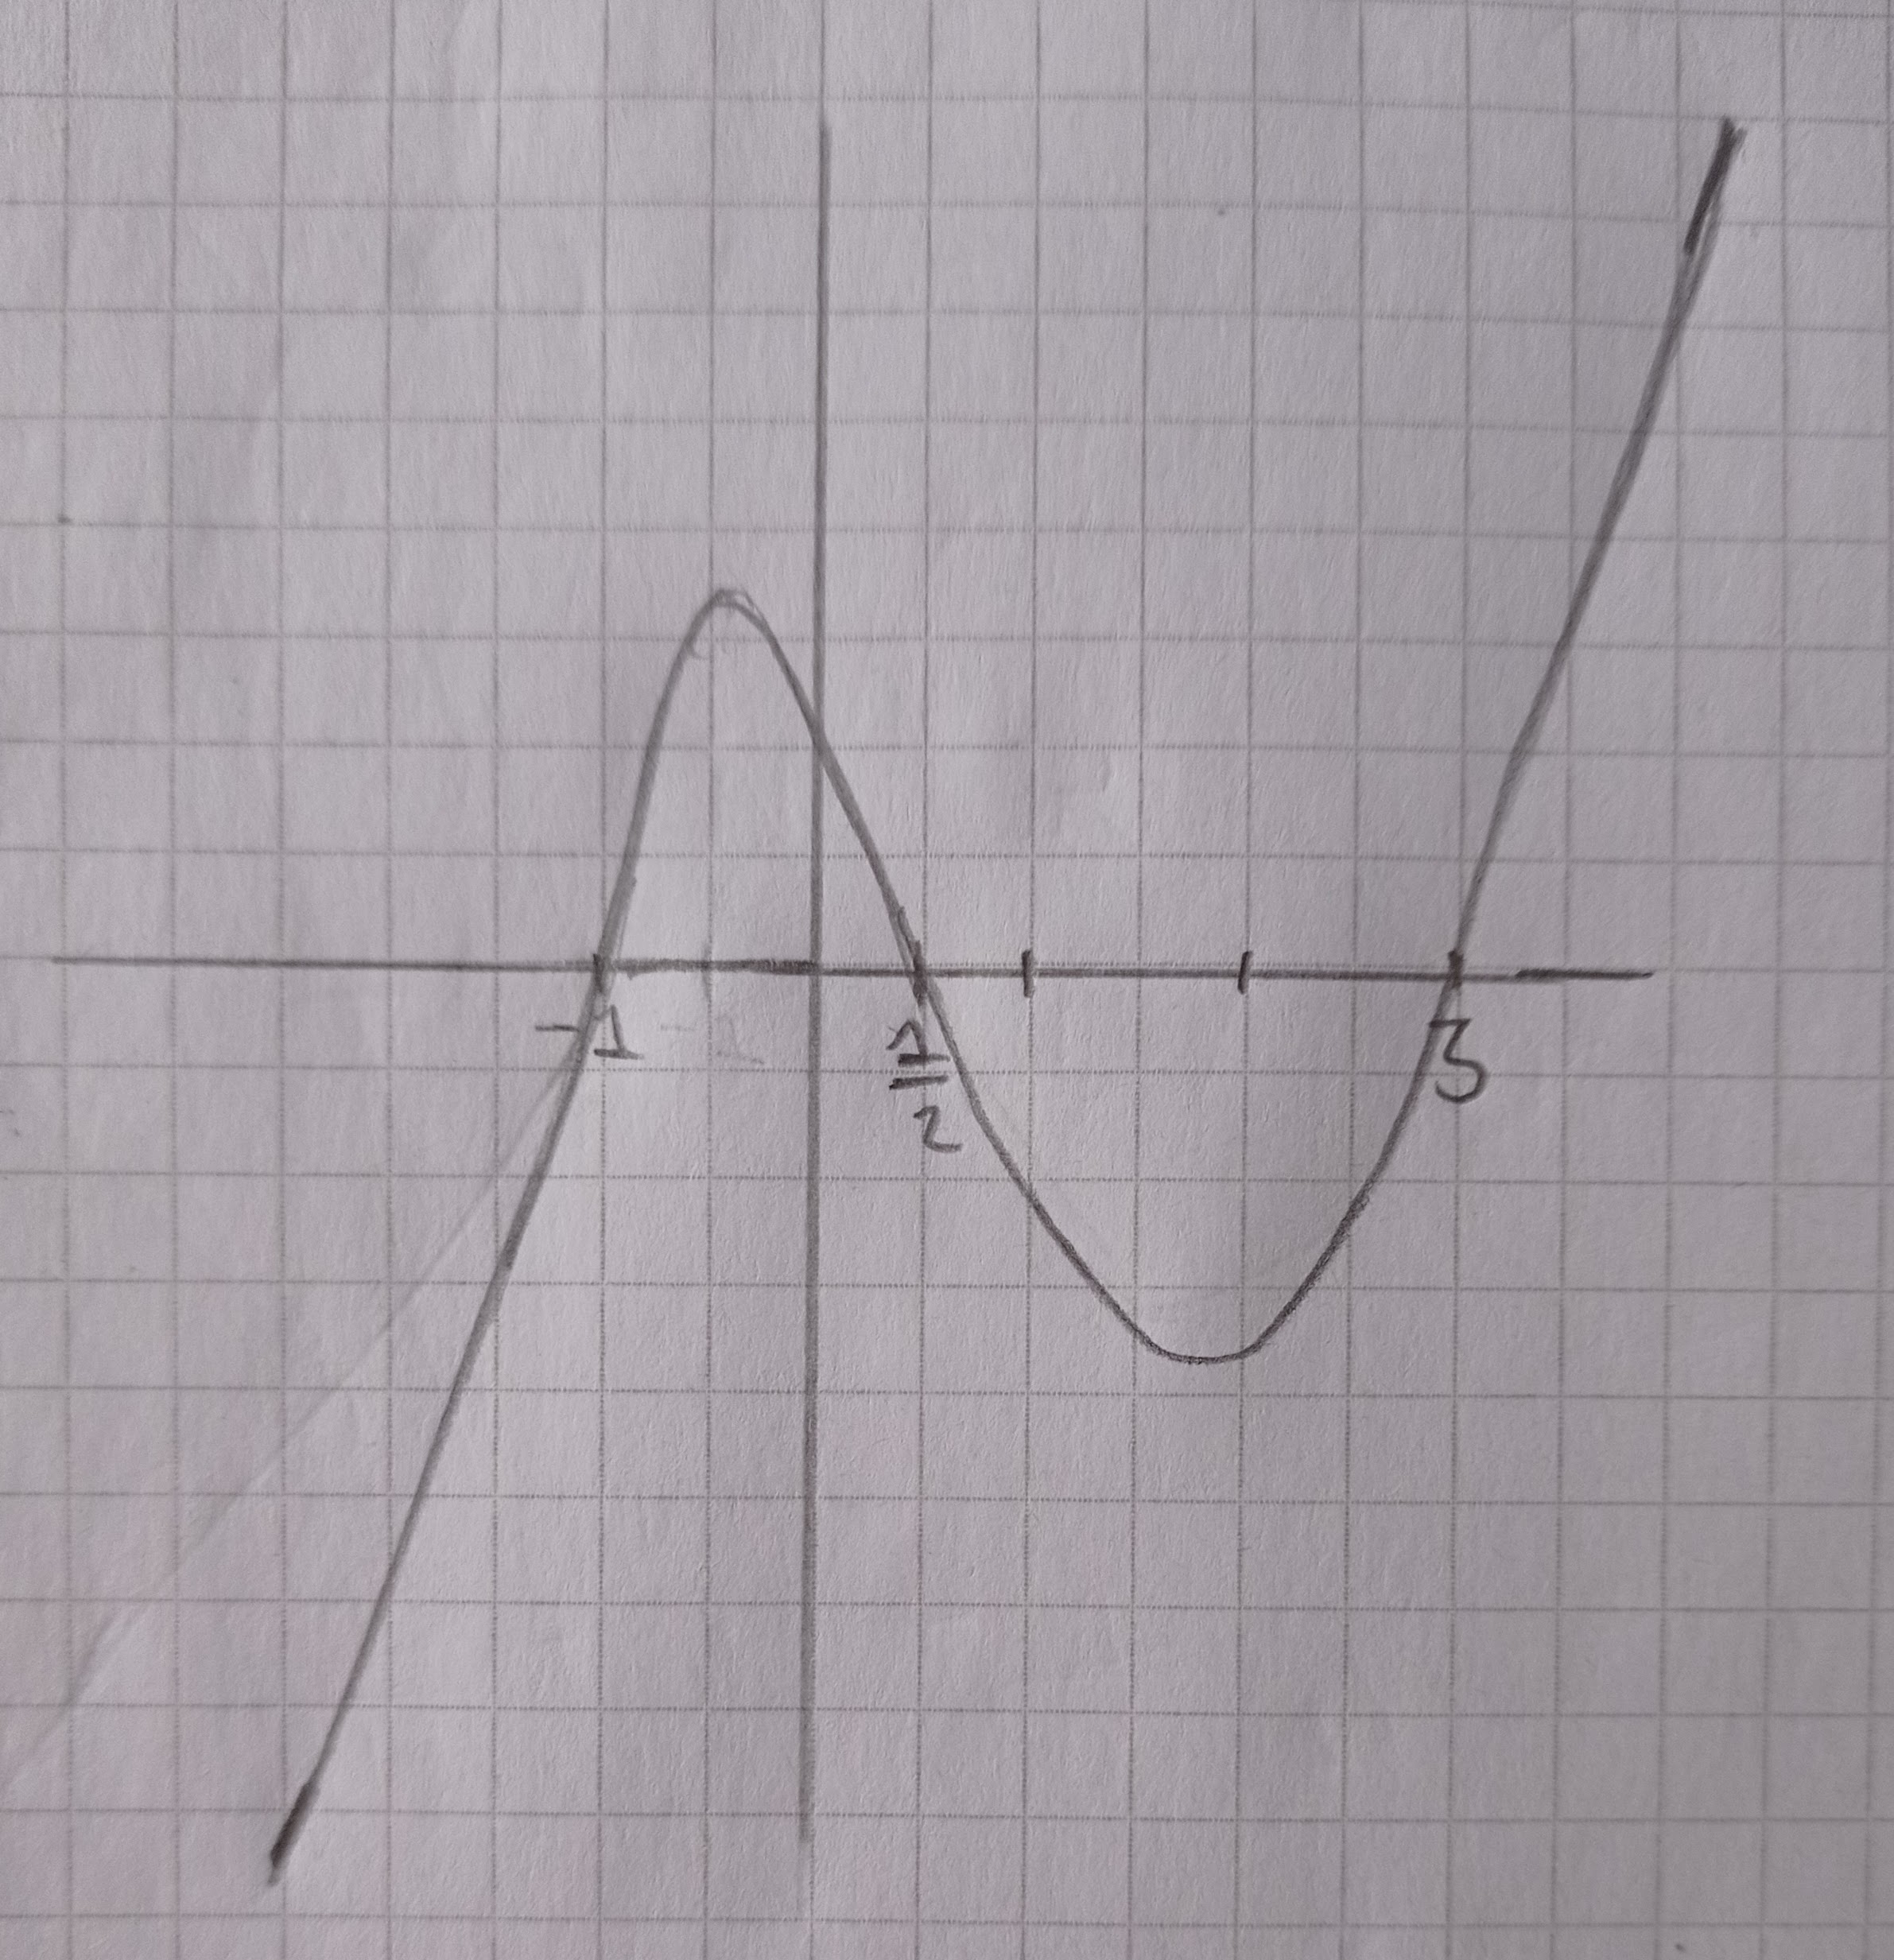
\includegraphics[height=4cm]{images/foto1.jpg}
                \end{center}
        \end{enumerate}
    \section*{Complejos}
        Sea $z=3-2i, w=4 +3i$. Halle.

        \begin{enumerate}
            \item $zw$
                \begin{align*}
                    zw &= (ac - bd) + (ad + bc)i\
                    &= (3 \cdot 4 - (-2 \cdot 3)) + (3 \cdot 3 + (-2 \cdot 4))i
                    &= 18 + i
                \end{align*}
            \item $\frac{z}{w}$\\
                $\frac{3-2i}{4+3i} \cdot \frac{4-3i}{4-3i} = \frac{18-17i}{16 + 9} = \frac{18-17i}{25} = \frac{18}{25} - \frac{17}{25}i$
            \item Encuentre los ceros reales y complejos de $P(x) = x^3 - x^2 -4x -6$.\\
                Usando el teorema de las raices racionales y división sintética encontramos que $3$ es un cero del polinomio. Luego el polinomio restante de la división es $x^2 + 2x +2$. Usando la fórmula cuadrática tenemos que los ceros restantes son los siguientes.
                \begin{align*}
                    & x=\frac{-2\pm\sqrt{(2)^2-4(1)(2)}}{2(1)} \\
                    & x=\frac{-2\pm\sqrt{-4}}{2} \\
                    & x=-1\pm i \\
                    & x_1=-1+i \\
                    & x_2=-1-i
                \end{align*}
                Por lo tanto las raices del polinomio son $3, -1 -i, -1 +i$.

            \item Encuentre un polinomio de cuarto grado con coeficientes enteros que tiene ceros $3i$ y $-1$, con $-1$ de multiplicidad $2$.\\
                Sabemos que $-3i$ también es una raíz del polinomio, por lo cual la forma factorizada del polinomio es la siguiente.

                $$ (x+1)(x+1)(x-3i)(x+3i) $$\\

                Expandiendo la expresión tenemos.

                \begin{align*}
                    (x+1)(x+1)(x-3i)(x+3i) &= (x+1)(x+1)(x^2+9) \\
                    &= (x^2+2x+1)(x^2+9) \\
                    &= x^4+9x^2+2x^3+18x+x^2+9 \\
                    &= x^4+2x^3+10x^2+18x+9
                \end{align*}
        \end{enumerate}
        \section*{Funciones Racionales}
            Considere las siguientes funciones racionales:
            $$ r(x) = \frac{2x-1}{x^2-x-2}, s(x) = \frac{x^3+27}{x^2+4} $$

            \begin{enumerate}
                \item Grafique $r(x)$, muestre con claridad cualquier asíntota y los posibles cortes con los ejes. \\
                    Asíntota vertical para $r(x)$.
                    \begin{align*}
                        x^2-x-2&= 0 \\
                        (x-2)(x+1)&= 0\\
                        x_1 = 2\\
                        x_2 = -1
                    \end{align*}
                    Asintota horizontal para $r(x)$.\\
                    Como el grado del numerador es menor que el grado del denominador, la asíntota horizontal está en $y = 0$. Luego la gráfica quda de la siguiente manera.
                    \includegraphics[height=4cm]{images/photo2.jpg}
                \item Grafique $s(x)$, muestre con claridad cualquier asíntota y los posibles cortes con los ejes. \\
                    Asíntota vertical para $s(x)$.
                    \begin{align*}
                        x^2+4&= 0 \\
                        x^2&=-4\\
                        x &= \sqrt{-4}\\
                        x &= i\sqrt{4}\\
                        x &= \pm 2i
                    \end{align*}
                    Como el grado del numerador es mayor al del denominador, tiene asíntota oblicua.
                    Al realizar el algorítmo de la división tenemos que la asíntota oblicua está en $y=x$. La gráfica quedaría de la siguiente manera.

                    \includegraphics[height=4cm]{images/photo3.jpg}
            \end{enumerate}
\end{document}
